\documentclass[10pt]{article}

\usepackage[
    style=numeric,%alphabetic, 
    backend=bibtex,
    sorting=none
    ]{biblatex}
\bibliography{refs}{}


\title{Pizza Guy}
\date{\today}
\author{Giacomo Boldini, Alessio Diana, Federica Zaglio}

%\usepackage{geometry}
\usepackage{booktabs}
\usepackage{xcolor}
\usepackage{hyperref}
\hypersetup{
    colorlinks,
    frenchlinks=true,
    linkcolor={blue!50!black},
    citecolor={green!50!black},
    urlcolor={red!80!black}
}
\usepackage{amsmath}
\usepackage{cleveref}

\usepackage{graphicx}
\graphicspath{ {figures} }
\usepackage{caption}
\usepackage{subcaption}

\begin{document}

	\maketitle

	\begin{abstract}

		In this report, we will describe the Pizza Guy project. This project 
		aims to find the best possible schedule of a set of orders that
		minimizes the distance traveled by the deliverers in a evening of 
		work. Our solution is developed using a CLP(FD) model and implemented 
		in MiniZinc. All the remaing part of the project (data retrieving, cleaning
		and visualization) are done using Python.\\	
		In the \cref{Assignment} we will describe the problem and the goal
		we want to reach, in the \cref{Model} we will the describe the 
		model and the implementation, including some euristichs and symmetry breaking
		strategies. In the \cref{Results} we will describe the results and
		the possible search strategies. Finally, in \cref{sec:conclusions} we will 
		conclude that the main problem in the proposed model is the solving time,
		that quickly increases considering a number of orders greater than 10
		and a number of deliverers greater than 4, which are relatively small. 
		Also, some possible changes and improvements 
		will be proposed.
		
	\end{abstract}

	{
	\footnotesize
	\tableofcontents
	}

	\pagebreak

	\section{The problem}
	\label{Assignment}
	The main problem we want to solve can be described as follow: the best pizzeria in the 
	town delivers pizzas at home; we want to find the best schedule of the set of orders 
	(for a single evening) that minimize the total traveled distance by the deliverers 
	respecting the delivery times requested by the customers.
	
	The assignment gives us the following informations about the problem:
	\begin{enumerate}
		\item an order consists of:
		\begin{enumerate}
			\item a delivery address;
			\item a desired delivery time;
			\item a number of pizzas;
		\end{enumerate}
		\item the desired delivery time has a granularity of 15 minutes (from 
			19.00 to 22.00);
		\item the delivery window is up to 30 minutes later than desired delivery 
			time;
		\item the street topology of the city can be seen as a graph: the nodes represent
			the addresses and they are connected by edges that contain travel time 
			between nodes; so, we know the distance (in terms of time) between each pair of addresses
			in the town;
		\item every deliverer can carry at most 16 pizzas;
		\item multiple travels from and to the pizzeria are allowed even in the 
			delivery window.
	\end{enumerate}

	To solve the problem means to assign a set of sorted lists of orders 
 	to every deliverer. Each list represents a travel and all the orders in it 
	must be handled (or, in other words, the destination of this order must be reached) 
	in the specified sequence.

	\subsection{Assignment}

	The goals of this work are:
	\begin{enumerate}
		\item write a program that solves the problem (in MiniZinc);
		\item write a benchmark suite using 5 different towns of increasing size
			and 10 input sets for each one; the input sets must enforce that all
			the deliverers do at least two travels (in \cref{subsec:test-5-cities})
		\item on one configuration that runs in a couple of minutes, try
			different search strategies and then use the most promising one to solve a
			difficult input set (in \cref{subsec:test-strategies}).
	\end{enumerate}

	\section{Model}
	\label{Model}

	%file: \texttt{an-idea-2.mzn}\\~\
	
	\subsection{Input data}

	\paragraph*{}
	The input consists in having:
	\begin{enumerate}
		\item $d$: the number of deliverers available
		\item $mdist$: the 2-d matrix representing the travel distance between
			every pair of nodes in the graph generated using Dijkstra (including those
			that are not a destination)
		\item $k$: the side dimension of $mdist$
		\item a set of $N$ orders, each of them made by a destination $dest$, a delivery 
			time $orario$ and a number of pizzas $num\_pizzas$

			\begin{equation*}
				\begin{split}
					\text{orario} &= [o_1, o_2, \dots, o_N];\\
					\text{num\_pizzas} &= [np_1, np_2, \dots, np_N];\\
					\text{dest} &= [d_1, d_2, \dots, d_N];
				\end{split}
			\end{equation*}

			%TODO: cambiare il nome della struttura dati "ORARIO"
	\end{enumerate}

	\subsection{Assumptions}
	\label{subsec-assumptions}
	In order to make the problem a little easier, we made the following 
	semplifications:
	\begin{enumerate}
		\item the graph is undirected, so \texttt{mdist} is symmetric:
		\begin{center}
			\texttt{mdist[x, y] = mdist[y, x]}
		\end{center} 
		As we'll show later, we can use Dijkstra on a real-world graph to calculate 
		distances between the nodes. In this case, \texttt{mdist} matrix could be
		asymmetric. 

		\item a deliverer can do only a single travel in one half-an-hour. In other
			words, the orders that are assigned to him/her are delivered creating 
			a circuit starting from the pizzeria, visiting all the destinations 
			and ending in the pizzeria in one half-an-hour;
		\item distances and travels time are considered the same thing;
		\item the set of orders is known before the start of the evening;
		\item all the time needed by the deliverer to interacts with customers (give them the pizzas,
			eventually handle the payment and other stuff) is supposed to be zero. %upon delivery
	\end{enumerate}

	\subsection{Implementation}


	%\textbf{TODO:} 
	%\begin{itemize}
	%	\item Scrivere di sched, P, dist che hanno le stesse pos valorizzate.
	%	\item Def. da minizinc
	%	\item Spiegare che tante cose servono per semplificare i calcoli
	%\end{itemize}
	
	The time is divided in 6 slots of half-an-hour (19.00 - 22.00). Let's call
	$h$ one of these slots of time.
	There are $d$ deliverers available for doing deliveries.
	Each deliverer, $d$, has a set of orders to handle for each slot of time $h$.

    \paragraph*{Scheduling}
	These informations are stored in a boolean 3-d matrix called 
	\texttt{scheduling} in which: 
	
	\begin{center}
		\texttt{scheduling[$d$, orderID, $h$] = true}
	\end{center}
	
	means that the deliverer $d$ has to deliver the order with id 
	\texttt{orderID} in the time slot $h$. In every slot $h$, the deliverer must 
	reach all nodes specified as \textit{destinations} (\texttt{dest}) of the orders assigned to 
	him/her, starting from node $1$ (pizzeria) and returning back to it. This creates
	 a sort of \textit{circuit} starting and ending with the same node, that reaches all the 
	nodes specified in the matrix row.

	Obviously, one order can be delivered only once during the evening by only
	one deliverer, and must be done in the delivery window computed from the requested time.

	\begin{center}
		\texttt{array[1..d, 1..N, 1..h] of var bool: scheduling;}
	\end{center}

	\paragraph*{Pizzas\_carried}
	During the evening there are $N$ orders to be delivered, each of which is made of
	16 pizzas at most. This ensure that we need only a deliverer to deliver the 
	entire order.
	Since we can deliver more than one order in a single travel, we need to
	record the total number of pizzas that a deliverer has in his/her bag.
	To do this, we use a 2-d matrix called \texttt{pizzas\_carried} where
	the first dimension represents the deliverer $d$ and the second 
	represents the half-an-hour $h$ considered.


	\begin{center}
		\texttt{array[1..d, 1..h] of var 0..16: pizzas\_carried;}
	\end{center}

	\paragraph*{Ea - Estimated arrival}
	In order to ensure that all deliveries arrive in time, we use \texttt{ea} which
	stands for estimated arrival. This array contains, for every order, the arrival 
	time (in minutes) from the starting time (19.00). At every order, we sum the number 
	of minutes that must pass before the delivery take place, so doing this way,
	we are sure that the delivery is done in the right delivery window.
	For example, if the delivery is requested for 20.00, if the destination is five minutes 
	far from the pizzeria and no other delivery is made before that, we will sum 60 to 
	be sure about the right delivery window and 5 for the travel time. So the \texttt{ea}
	for this delivery will be 65.
	
	\begin{center}
		\texttt{array[1..N] of var 0..h*30: ea;}
	\end{center}
	

	\paragraph*{P} The main goal of the project is to minimize the travel distance 
	covered by all the deliverers in the evening. To do so, a possible strategy
	is to deliver more than one delivery in a single travel. This is convenient 
	if the deliveries are made in a way that minimize the distance traveled between the nodes.
	To encode this information, we use \texttt{P}, which is a 3-d matrix that stores
	all the nodes that every deliverer has to visit in one travel, according to \texttt{scheduling}. 

	\begin{center}
		\texttt{array[1..d, 1..N, 1..h] of var array2set(dest) union {0}: P;}
	\end{center}
	%The useful thing
	%about this matrix is that it allows us to control the order of each delivery made 
	%by every deliverer in one travel and compute the travel distance.
	
	\paragraph*{X} This 3-d matrix is used to support the creation of all the other 
	constraints, making the computation of the distances easier.
	In this matrix, meangingful \textit{positions} of the matrix $P$ are stored for each 
	$d$ and $h$. Each row contains the positions of the matrix P (destination nodes) 
	that $d$ deliverer has to reach in the $h$ half-an-hour. This matrix allows 
	us to control the order of each delivery made by every deliverer in one travel
	and, as consequence, compute the corresponding travel distances (stored in \texttt{distances}).

	\begin{center}
		\texttt{array[1..d, 1..N, 1..h] of var 0..N: X;}
	\end{center}
	% magari un esempio non sarebbe male

	\paragraph*{Distances}
	Using the data structures seen before, we use this 3-d matrix to store all
	the partial distances needed to reach every delivery node starting from 0 for each
	half-an-hour. Using this matrix we can enforce that all the deliveries are delivered in 
	time and, since we want to minimize the traveled distance, it allows us to combine deliveries that belongs to different
	time slots (eg. 19.15 and 19.30) but only if they are adjacent because of the maximum 
	delivery time of 30 minutes.

	\begin{center}
		\texttt{array[1..d, 1..N, 1..h] of var 0..29: distances;}
	\end{center}

	\paragraph*{}
	The matrices $scheduling$, $P$ and $distances$ are strictly related to each other.
	They encode the same concept but using different informations. First of
	all they have the same sizes \texttt{[1..d,1..N,1..h]} and if one cell is meaningful in
	one	of them, it is also meaningful in the others.
	In particular, in a position 
	\texttt{[id,iN,ih]}:
	\begin{itemize}
		\item \textit{sheduling = 1} means that the order \textit{iN} has to be
		accomplished by the deliverer \texttt{id} in the \texttt{ih} half-an-hour;
		\item \textit{P = n} means that the order \textit{iN} has to be
		accomplished by the deliverer \texttt{id} in the \texttt{ih} half-an-hour 
		reaching the node \texttt{n} in the graph;
		\item \textit{distances = l} means that the order \texttt{iN} has to be
		accomplished by the deliverer \texttt{id} in the \texttt{ih} half-an-hour 
		and it will take $l$ minutes to reach it, starting from the beginning of the
		corresponding half-an-hour (partial time).
		 
	\end{itemize}
	All the others meaningless positions are set to zero in all the matrices.

	\paragraph*{Total\_travel}
	We use this 2-d matrix in order to store the total travel distance of deliverer \textit{id} in one half-an-hour \textit{ih}.
	As described above, in the matrix \textit{distance} there are partial distances: from pizzeria for each delivery node handled,
	starting from the corresponding half-an-hour.
	If we add the distance between the last delivery node and the pizzeria (that is the path to return to the pizzeria)
	we have the total travel distance.
	As already mentioned, our goal is minimize the sum of all these values.

	\begin{center}
		\texttt{array[1..d, 1..h] of var 0..29: total\_travel;}
	\end{center}

	\subsection{Constraints}

	To ensure \texttt{scheduling} consistency, the following constraints are made:
	\begin{itemize}
		\item \texttt{sum(scheduling) = N;} ensures that all the orders are fulfilled %and
		\item \texttt{forall(j in 1..N)(\\
			sum([scheduling[id,j,ih]| id in 1..d, ih in 1..h]) = 1\\
		  );} ensures that only one delivever takes care of one order. 
	\end{itemize}

	\paragraph*{}
	To construct the matrix \texttt{P} a simple product between a \texttt{scheduling} row and the array of the destinations \texttt{dest} is
	made:
	\begin{verbatim}
forall(id in 1..d, iN in 1..N, ih in hra[iN])(
   P[id, iN, ih] = scheduling[id, iN, ih] * dest[iN]
);
	\end{verbatim}
	
	Thanks to this product, we are able to make meangingful the same positions
	of \texttt{scheduling}.

	\paragraph*{}
	The \texttt{X} matrix has to contain all the meaningful	positions in the matrix
	\texttt{P}. To ensure this, we need a simple way to sequentially compute all the
	informations related in a single row. For every value greater than zero found in a row 
	of \texttt{P}, we enforce the corresponding row of \texttt{X} to contain it. 
	Also, we want to push all the meaningless values (zeros) to the end of the row: this is done
	by another constraint described below (\cref{subsubsec:restrict-search-space} (3)).	

	\begin{verbatim}
forall(id in 1..d, iN in 1..N, ih in 1..h)(
   if P[id, iN, ih] > 0 then 
      count([ X[id, iNN, ih] | iNN in 1..N], iN, 1)
   else
   (
      count([ X[id, iNN, ih] | iNN in 1..N], iN, 0) 
      /\
      distances[id,iN,ih] = 0
   )
   endif
);
	\end{verbatim}


	\paragraph*{}
	To compute distances means to fill the \texttt{distances} matrix.
    To do this, we have to use the matrix \texttt{X}. 
	Considering a single row, we must take care of the following cases:
	\begin{itemize}
		\item the first (meaningful) cell;
		\item the other (meaningful) cells.
	\end{itemize}
	
	
	In the first case, if \texttt{X[1]} is the first meaningful position in the 
	matrix P and \texttt{P[X[1]]} is the first visited node in a travel,
	the distance of the node \texttt{P[X[1]]} is computed summing the 
	distance between the pizzeria (node number 1) and this node: \texttt{mdist[1, P[X[1]]]}.
	This value is put in \texttt{distances[X[1]]}.\\
	
	In the second case, the distance to reach the node in \texttt{X[i]} is 
	the sum of the distance between the node \texttt{X[i]} and \texttt{X[i-1]}, and the last 
	distance previusly computed (\texttt{distances[X[i-1]]}). 
    % TODO: DA SCRIVERE IN MATEMATICHESE!! COME DICE MINOOO!!! 
	
	For the sake of simplicity, in the example above, the matrices \text{P} and \text{X} are treated 
	like arrays to avoid writing all the other indexes that are fixed because we are considering a single 
	row.

	
	\begin{verbatim}
forall(id in 1..d, iN in 1..N, ih in 1..h)(
   if X[id,iN,ih] !=0 then
      if iN == 1 then
         distances[id, X[id,iN,ih], ih] = 
            mdist[1, P[id, X[id,iN,ih], ih]] 
       else
          distances[id, X[id,iN,ih], ih] = 
            mdist[P[id, X[id,iN-1,ih], ih], P[id, X[id,iN,ih], ih]] 
         	+ distances[id,X[id,iN-1,ih], ih]
                  | iNN in 1..iN-1])
       endif
   endif
);
	\end{verbatim}

	\paragraph*{}
	Moreover, using \texttt{X}, we must check the "travel consistency", which 
	means that the deliverer must be able to return back to the pizzeria before the 
	start of the next half-an-hour. 
	To do this, we store the computed travel distance in \texttt{total\_travel} and its 
	domain \texttt{[0..29]} ensures this property.  

	\paragraph*{}
	To make \texttt{ea} consistent, which is the array that allow us to record the expected arrival
	time of each delivery, we take into account the row representing the delivery in the 
	\texttt{scheduling} matrix and the same position in the \texttt{distances} matrix. Since 
	\texttt{scheduling} is a boolean matrix, only the meaningful position in 
	\texttt{distances} will be used. For every half-an-hour from the starting time to the 
	beginning of the corresponding half-an-hour, 30 is added to this value. 
	In addition, we must constraint that every delivery is delivered within 
	30 minutes starting from the desired delivery time.
	\begin{verbatim}
forall(iN in 1..N)(
   ea[iN] = sum([scheduling[id,iN,ih]
            * (distances[id,iN,ih]+((ih-1)*30)) 
               | id in 1..d, ih in 1..h])
   /\
   ea[iN] >= ra[iN] 
   /\ 
   ea[iN] < ra[iN]+30 
);
	\end{verbatim}


	\paragraph*{}
	The consistency of \texttt{pizzas\_carried} is trivial. For every order, we enforce that the 
	number of pizzas carried by a deliverer in one half-an-hour is the same as the number of 
	pizzas in the orders that he/she is taking care of in the same half-an-hour.
	\begin{verbatim}
forall(id in 1..d, ih in 1..h)(
   pizzas_carried[id, ih] = sum([ num_pizze[j]
                                | j in 1..N 
                                where scheduling[id, j, ih] = 1])
);
	\end{verbatim}

	\paragraph*{}
	Some of the data structures previously analized could have been avoided if we 
	wanted to have a more lightweight model. We introduced them to make simpler the
	creation of the constraint and to keep the model readable.
	
	% SCEGLIERE SE SCRIVERE CHE NON SAPPIAMO SE L'AUMENTO DELLE STRUTTURE CHE 
	% VENGONO UTILIZZATE NEL MODELLO POSSA AVER PEGGIORATO LE SUE PRESTAZIONI GLOBALI 

	\subsubsection{Restrict the search space}
	\label{subsubsec:restrict-search-space}
	Creating the model, we included some easy euristichs that can restrict the dimension
	of the search space:

	\begin{enumerate}

		\item domain restrictions.
		
		As said in \cref{Model}, the domain for each decision variable has been
		strictly restriced to the only possible values that they can assume. 
		For example, a cell of \texttt{distances}, that represent the partial travel time
		to reach a destination, can't be greater than 29 since we want that each deliverer 
		returns back to the pizzeria before the next half-an-hour. Another example is the domain
		of \texttt{P}: in this case we restrict the domain from \texttt{0..k} (which is correct) 
		to only the set of possible destinations. This reduces a lot the number of possibility in 
		the domain. 

		\item for each order, exclude all the non-possible half-an-hour.
		
		Every order has a requested delivery time that becomes a delivery window. 
		We know that all the half-an-hours before and after this delivery window
		are not usable. So, for each order we computed its \textit{valid} half-an-hour 
		indeces (\texttt{hra}) that are used to access the matrices \texttt{scheduling}
		and \texttt{P} in \textit{not-valid} half-an-hour to set it equal to zero.   
		Also, a consideration on \texttt{X} matrix is made: for each \textit{not-valid} 
		half-an-hour for a specific order, we know that this order index will be not present
		in the corresponding row of \texttt{X}.

		%\textbf{maybe distances}

		\begin{verbatim}
forall(id in 1..d, iN in 1..N, ih in (1..h diff hra[iN]) ) (
   scheduling[id,iN,ih] = 0
   /\
   P[id,iN,ih] = 0
   /\
   count( [X[id,iNN,ih] | iNN in 1..N], iN, 0)
);
		\end{verbatim}

		\item enforce useless cells of matrix \texttt{X} to zero.
		
		Each line of \texttt{X} contains the indexes of the corresponding line of \texttt{P}
		that are meangingful (different from zero). Also, all the zero in this (\texttt{X}) 
		line must be pushed to the end of it. Knowning this, if we count the number of zeros
		in each line of \texttt{P} we can contraint the same number of cells to be zero, starting
		from the end of line of \texttt{X}.

		\begin{verbatim}
forall(id in 1..d, ih in 1..h)(
   let {
      var int: c = count([P[id,iNN,ih] | iNN in 1..N],0)
   }
   in forall(iN in N-c+1..N)(
      X[id,iN,ih] = 0
   )  
);
		\end{verbatim}
		

	\end{enumerate}

	\subsubsection{Simmetry breaking strategy}
	Having more than one deliverer implies the possibility of having the same solution 
	multiple times. For example, if we have three delivery and two deliverers, known that
	the best strategy is to deliver the first two togheter and the third alone, one solution is 
	to give the first two to the deliverer \texttt{d1} and the third to the deliverer \texttt{d2}.
	A simmetric and equivalent solution is to give the first two to \texttt{d2} and 
	the third to \texttt{d1}.

	In order to avoid this kind of problem, we impose an ordering on the deliverers by 
	counting the number of pizzas that are carried in one half-an-hour. This enforce that 
	the first deliverer carries a number of pizzas greater or equal to the number of
	pizzas carried by the second deliverer, the second deliverer a number of pizzas greater or 
	equal to the number of pizzas of the third deliverer and so on.
\begin{verbatim}
forall(ih in 1..h, id in 1..d-1)(
   pizzas_carried[id,ih] >= pizzas_carried[id+1,ih]
);
\end{verbatim}

%
%	\paragraph*{???}
%	As said before, the data structures used in the model are, in some way, redundant
%	to have a better readability. We are not sure if having a lower number of data 
%	structures and a more complex constraint generation would have made the model
%	faster in finding the best solution.
%
	\section{Results}
	\label{Results}

	In this section, we will describe how the model behave, mainly in terms of solving
	time, using different input data and different search strategies.

	To do this, we consider 5 italian city of increasing size (listed by increasing dimension): 
	\textit{Visano(BS)}, \textit{Asola(MN)}, \textit{Montichiari(BS)}, \textit{Brescia (BS)} and \textit{Roma (Roma)}.
	Their street graphs have the following characteristics:%features:
	\begin{table*}[h]
		\centering
		\begin{tabular}{l|ll}
			City & nodes & edges \\
			\hline
			Visano & 297 & 378 to\\
			Asola & 480 & 664 \\
			Montichiari & 1130 & 1509 \\
			Brescia & 3925 & 5464 \\
			Roma & 4729 & 7277 \\
		\end{tabular}		
	\end{table*}
	
	As preprocessing step, for each of them we computed the shortest path beetween all the pairs
	of nodes using Dijkstra. This produced the corresponding $mdist \in M^{nodes \times nodes}$.
	%For assumption (2) in \cref{subsec-assumptions}, these matrices are symmetric.

	In addition to the model tests, we report a \textit{real-world} result of a model execution, obtained using some pre- and post-processing techniques.  

	\subsection{Search strategies comparison}
	\label{subsec:test-strategies}
	Choosen a configuration of the problem that runs in a couple of minutes,
	we tested how it performs (in terms of solving time) changing the search strategies.
	The configuration choosen is:
	\begin{center}
		$N = 12$ (orders), $d = 2$ (deliverers), city = Visano.		
	\end{center}

	First of all we made a preliminary analysis, which results are shown in
	\cref{subsubsec:preliminary-analysis}. Then, more specific analyses
	are made on a subset of possible search strategies (the most promising among all)
	and results are shown in \cref{subsubsec:more-specific-analysis}.

	The best strategy we found in the preliminary analysis (in terms of solving time) is the one shown
	in \cref{tab:best-strategy}. However, as we found later, searching on variable \texttt{P}
	isn't the optimal one (on average). 
	Indeed, later we used the \texttt{scheduling} variable, which turned out to be 
	the best one (on average).

	\begin{table*}[h]
		\centering
		\scriptsize
		\begin{tabular}{ll}
			\toprule
			var          &                P \\
			vsa          &  anti\_first\_fail\\
			vca          &         indomain \\
			\midrule
			initTime     &         0.665783 \\
			solveTime    &          4.45827 \\
			solutions    &              2.0 \\
			variables    &           5925.0 \\
			propagators  &           2322.0 \\
			propagations &        2118705.0 \\
			nodes        &           5179.0 \\
			failures     &           2916.0 \\
			restarts     &              0.0 \\
			peakDepth    &             18.0 \\
			\bottomrule
		\end{tabular}
		\caption{Search strategy with minimum solve time in preliminary analysis.}
		\label{tab:best-strategy}
	\end{table*}

	

	\subsubsection{Preliminary analysis}
	\label{subsubsec:preliminary-analysis}
	
	First of all, we made preliminary analyses to figure out the most promising
	search strategies among all their possibile configurations. To do this,
	we simply analyzed the variation of solving time changing the search 
	annotations in Minizinc: in particular, we changed (1) the search 
	variable, (2) how the variable is choosen and (3) how to constraint
	the variable. \\Results are shown in \cref{fig:search-strategies-gen} 
	and we can see that searching of variable \texttt{scheduling} could be 
	the faster choice. Also, some VCA (Variable Choice Annotation) and VSA 
	(Variable Search Annotation) appear to be more promising than others. 




	\begin{figure}
		\centering

		\begin{subfigure}[c]{\textwidth}
			\centering
			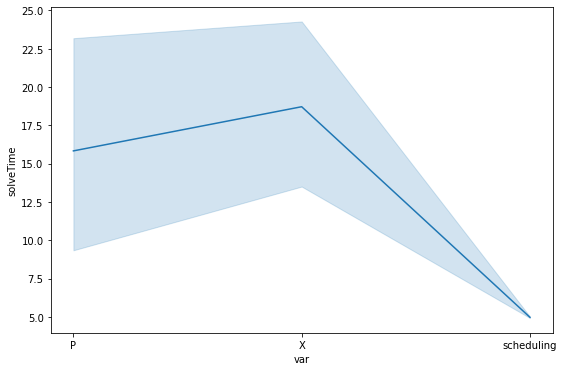
\includegraphics[width=.5\textwidth]{var.png}
			\caption{changing search variable.}
		\end{subfigure}
		\begin{subfigure}[b]{\textwidth}
			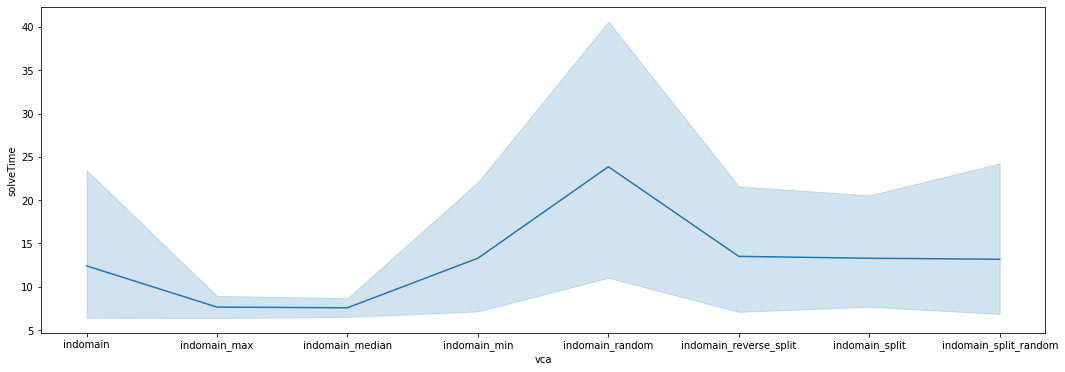
\includegraphics[width=\textwidth]{vca.png}
			\caption{changing Variable Choice Annotation (VCA)}
		\end{subfigure}
		\begin{subfigure}[b]{\textwidth}
			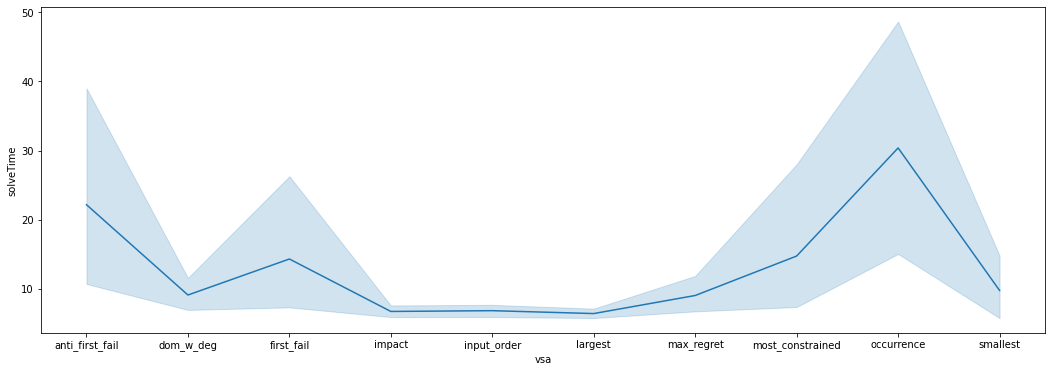
\includegraphics[width=\textwidth]{vsa.png}
			\caption{changing Variable Search Annotations (VSA)}
		\end{subfigure}
		
		\caption{How solving time behave (on average) changing search strategies configurations.}
        \label{fig:search-strategies-gen}
	\end{figure}


	\subsubsection{More specific analysis}
	\label{subsubsec:more-specific-analysis}
	In this case, we selected a subset of search strategies (the most promising)
	and then we made a more specific analysis, reducing the timeout to 20 seconds 
	and testing the same strategy more than one single time. All the executions
	that reached the timeout are removed from the analysis.

	We computed the correration matrix (\cref{fig:corr}) between search statistics
	and it shows high correration between:
	\begin{itemize}
		\item number of failures and number of nodes ($1$);
		\item number of propagations and solve time ($0.79$): this, in addition to the non-correration
			between maximum depth and solve time ($-0.05$), points out that as the number of
			propagations increases, it also increases the solve time, but not the tree's depth.
			% Questo ci fa pensare al fatto che avere alberi larghi rispetto che profondi aumenti il tempo di esecuzione genereale(???? ipotesi)
			% Forse il nostro problema ci da subito delle soluzioni, ma non quelle ottime (e quindi bisogna far passare tutta la larghezza).
	\end{itemize}

	\begin{figure}
		\centering
		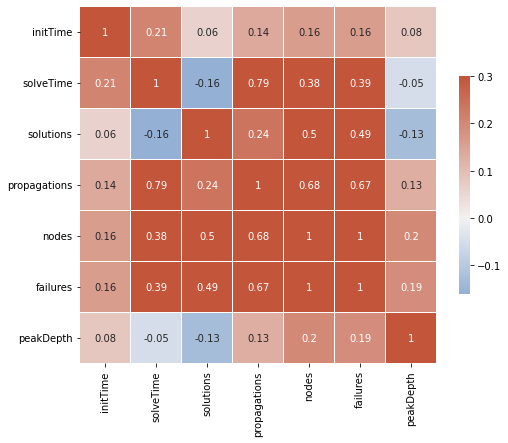
\includegraphics[width=.6\textwidth]{corr.png}
		\caption{Correlation matrix between the search statistics.}
		\label{fig:corr}
	\end{figure}

	In \cref{fig:solve-time-specific} more detailed solve time analyses are
	reported, for each search variable. It's clear that:
	\begin{itemize}
		\item regardless of which 
		VCA and VSA are choosen, searching on \texttt{scheduling} variable is faster
		than searching on \texttt{X} or \texttt{P} variables (again, on average).  
		\item searching on \texttt{scheduling} variable never leads to timeout executions.
	\end{itemize} 

	The \cref{tab:more-specific} shows a summary of these informations. 

	\begin{table}
		\scriptsize
		\centering
		\begin{tabular}{lrrrrrrrr}
		\toprule
		var &  count &      mean &       std &      min &       25\% &       50\% &     75\% &       max \\
		\midrule
		scheduling &  280.0 &  5.3998 &  0.5834 &  4.7762 &  4.87248 &  5.4201 &   5.576 &   8.7637 \\
		X          &  240.0 &  9.2220 &  2.7396 &  5.8241 &  7.03597 &  8.7616 &  10.510 &  20.0438 \\
		P          &  251.0 &  9.4433 &  5.0247 &  4.9271 &  5.55710 &  6.4068 &  15.243 &  19.5353 \\
		\bottomrule
		\end{tabular}

		\caption{Solve time statistics}
		\label{tab:more-specific}
	\end{table}

	\begin{figure}
		\centering
		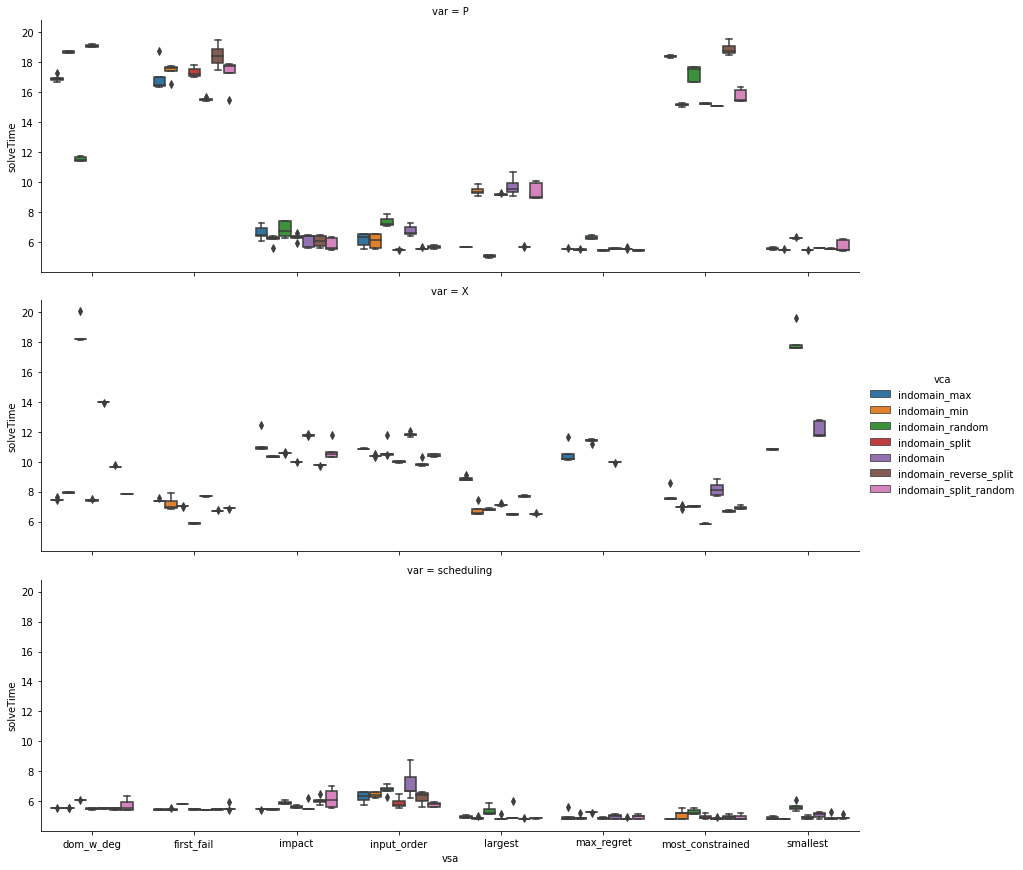
\includegraphics[width=\textwidth]{solve-time-specific.png}
		\caption{More specific analysis on solve time, changing the search strategies.}
		\label{fig:solve-time-specific}
	\end{figure}


	\pagebreak

	\subsection{5 city of increasing size}
	\label{subsec:test-5-cities}
	Using one of the best search strategies, we tried to solve the problem using all the 5 increasing 
	size cities in order to see how solving time changes. The timeout is set to 5 minutes for each execution.
	In this case, the configuration choosen is:
	\begin{center}
		$N = 12$ (orders), $d = 2$ (deliverers)	\\
		city = Visano, Asola, Montichiari, Brescia, Roma
	\end{center}
	Solving times found are shown in \cref{fig:city-increasing-size}. Solve and init times are 
	set to 300 seconds if the execution reached the timeout without solving the problem. This is the
	case for the two biggest cities (Brescia and Roma). For the other cities, the time increases
	with the size of the city and it is always under 20 seconds. 
	\begin{figure}
		\centering
		\begin{subfigure}[c]{.49\textwidth}
			\centering
			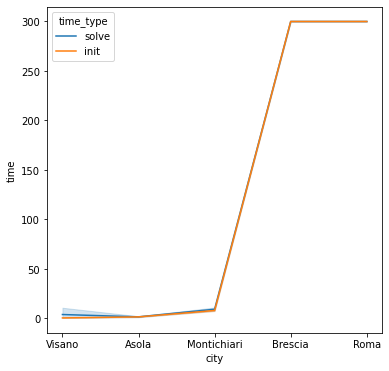
\includegraphics[width=\textwidth]{city-increasing-size.png}
			\caption{}
		\end{subfigure}
		\begin{subfigure}[c]{.49\textwidth}
			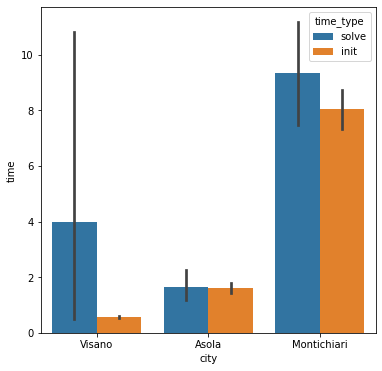
\includegraphics[width=\textwidth]{city-increasing-size-2.png}
			\caption{}
		\end{subfigure}

		\caption{Solving times for 5 cities of increasing size. $N = 12$, $d=2$}
		\label{fig:city-increasing-size}
	\end{figure}


	\subsection{Increasing the size of the problem}
	\label{subsec:test-size-of-problem}
	Using one of the best search strategies, we tried to solve a set of problems in the same city (Visano)
	with different complexities, represented by number of order $N$ and number of deliverer $d$. 
	The timeout is set to 2 minutes for each execution, $N$ ranges from $2$ to $15$ and $d$ ranges from $1$ to $4$. 
	Results are represented in \cref{fig:increasing-problem} and they show what we expected: the peak depth of
	the tree, the solve time, the number of solutions and propagations increases with $N$ and $d$. 
	
	\begin{figure}
		\begin{subfigure}[c]{\textwidth}
			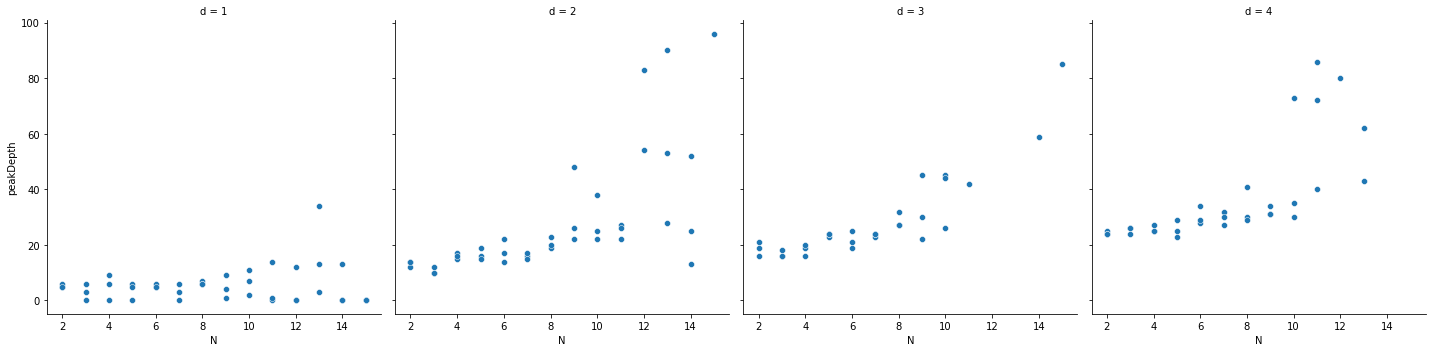
\includegraphics[width=\textwidth]{incr-problem-depth.png}
			\caption{peakDepth}
		\end{subfigure}
		\begin{subfigure}[b]{\textwidth}
			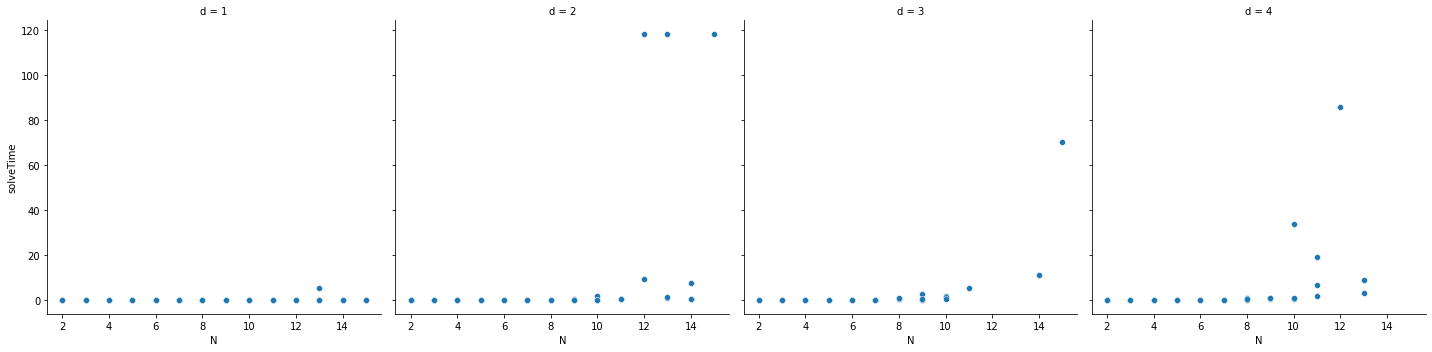
\includegraphics[width=\textwidth]{incr-problem-time.png}
			\caption{Solve time}
		\end{subfigure}
		\begin{subfigure}[b]{\textwidth}
			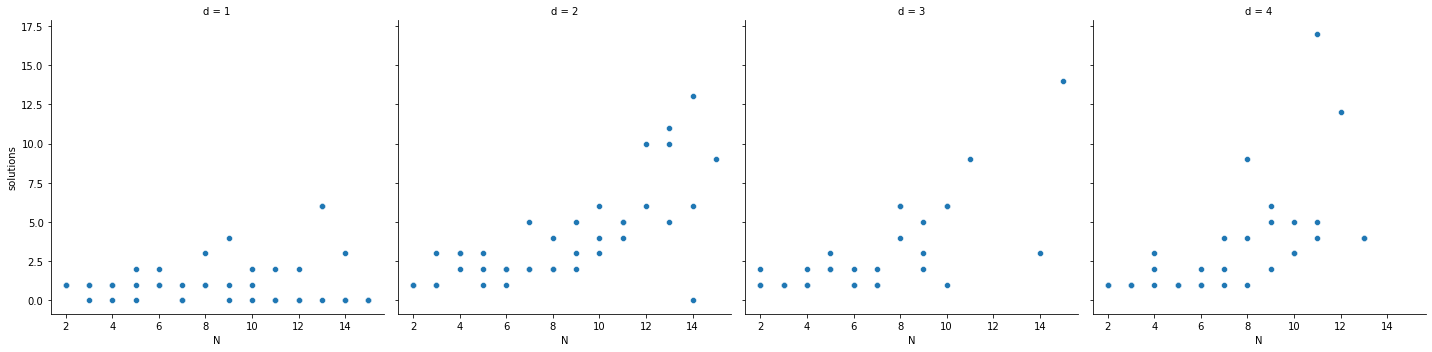
\includegraphics[width=\textwidth]{incr-problem-solutions.png}
			\caption{Solutions}
		\end{subfigure}
		\begin{subfigure}[b]{\textwidth}
			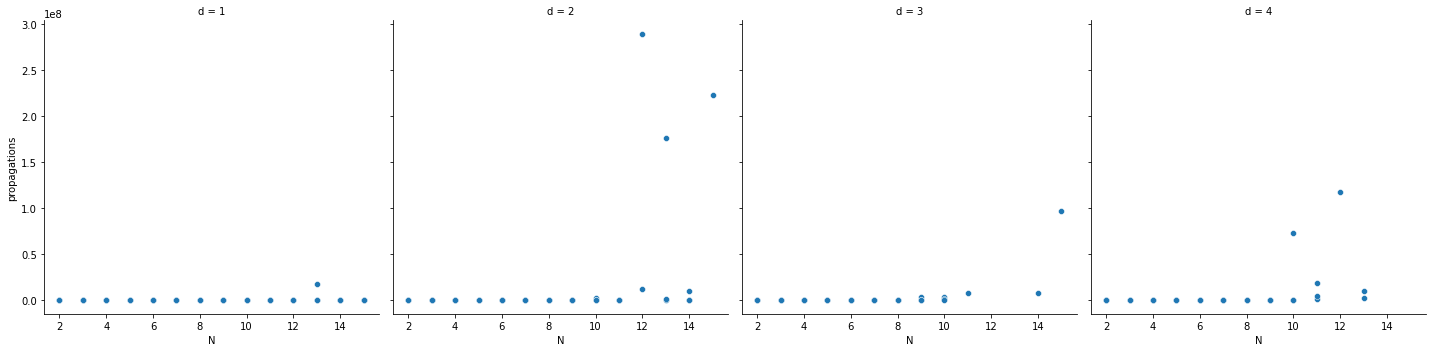
\includegraphics[width=\textwidth]{incr-problem-propagations.png}
			\caption{Propagations}
		\end{subfigure}

		\caption{Results increasing the size of the problem.
			$N = 2\dots15,\hspace{.5em} d=1\dots4$, city = Visano. 
			2 minutes timeout.}
        \label{fig:increasing-problem}
	\end{figure}

	\subsection{Real-world application}

	Using \textit{Python} and \textit{OpenStreetMap} we were able to execute the model
	on a graph obtained by a real-world map and plot the results directly on the streetmap.
	
	In \cref{fig:maps} there is an example of model execution on the city \textit{Visano}, 
	with $N = 13$ orders and $d = 2$ deliverer. Solve time was 48.8 seconds.

	\begin{figure}
		\begin{subfigure}[t]{.5\textwidth}
			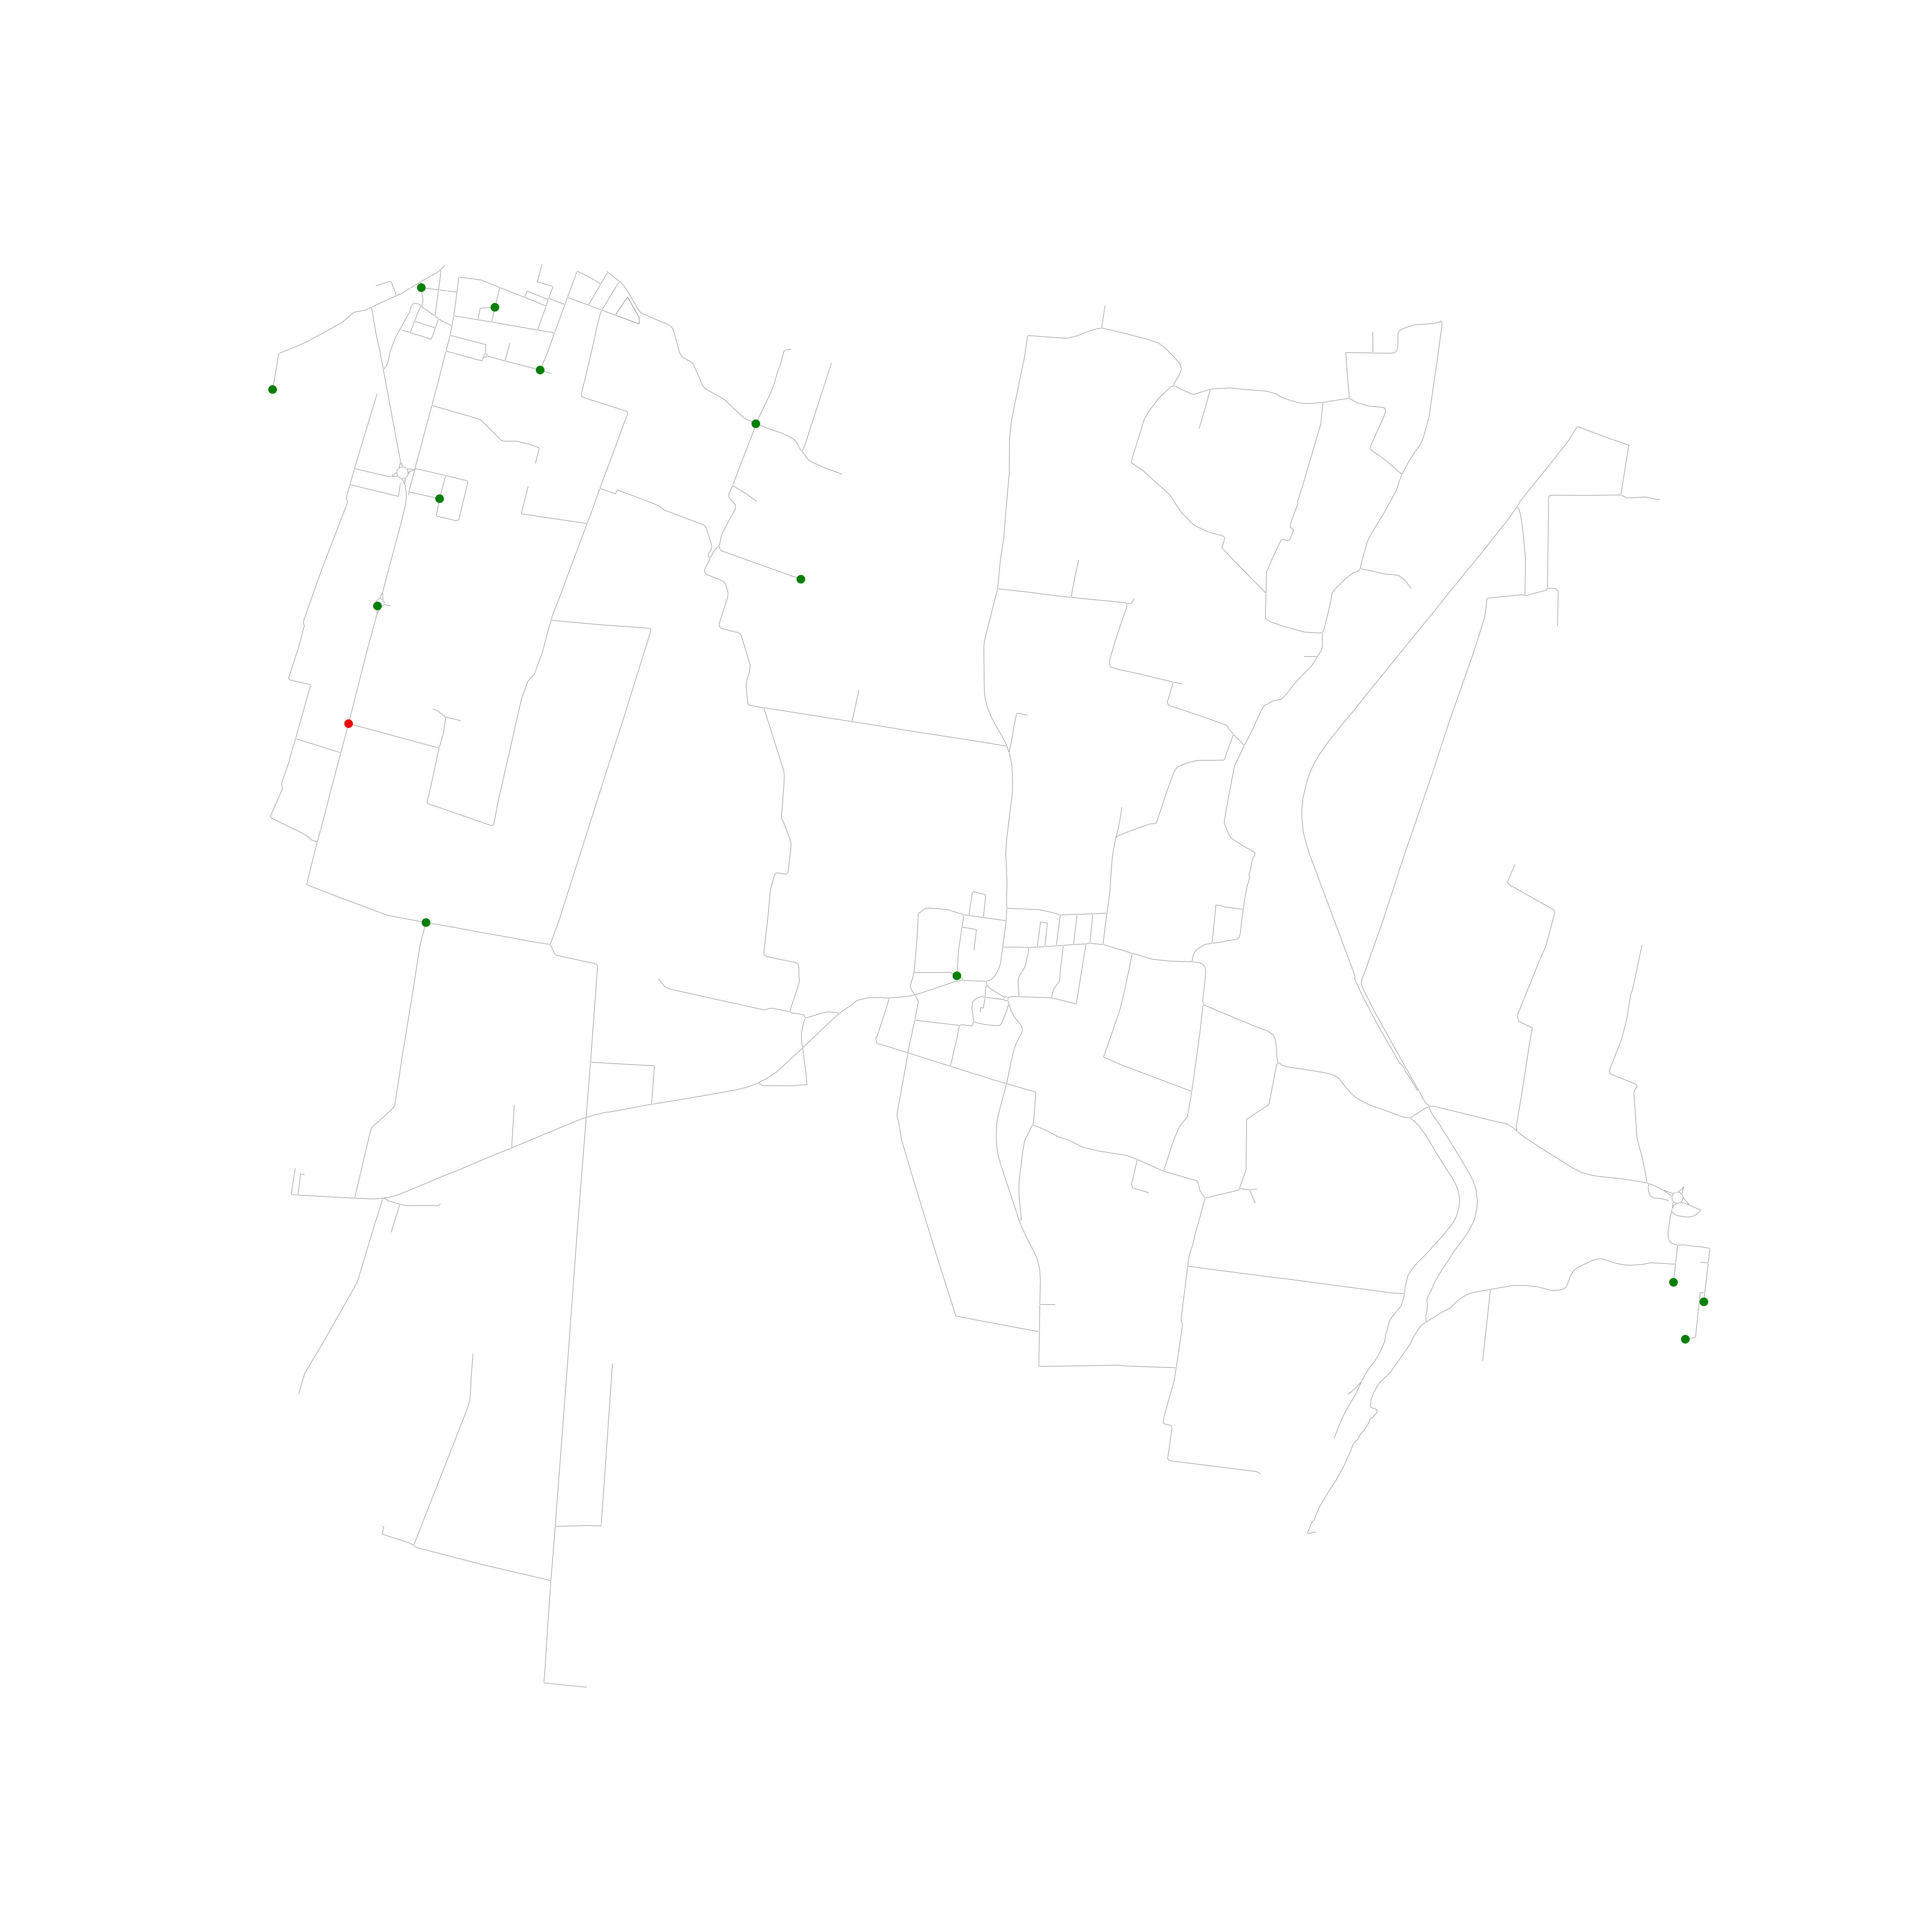
\includegraphics[width=\textwidth]{graph.png}
			\caption{Pizzeria (red) and destinations to reach (green)}

		\end{subfigure}
		\begin{subfigure}[t]{.5\textwidth}
			\includegraphics[width=\textwidth]{graph_paths-min.png}
			\caption{Path for each deliverer}
		\end{subfigure}

		\caption{Map plot of model's results.}
        \label{fig:maps}
	\end{figure}


	\section{Conclusions} 
	\label{sec:conclusions}
	Our proposed model seems to be working, \textit{but} the main problem is the solving time: 
	it increases quickly 
	with the size of the problem. Indeed, the model takes a couple of seconds to solve the problem
	only with a number of order $N \le 12$. Using a number of orders over this threshold, 
	the executions always reach the timeout of 5 minutes. With such a small value of $N$,
	we're far from a real world situation, which usually includes $N \ge 50$ (and more
	than $d = 3$ deliverer).

	Also, we tried to use different solvers (from Gecode), but we got no improvement; 
	on the contrary, we obtained worst results.

	One possible improvement that we tried is reducing \texttt{mdist} size, considering
	only the destination nodes.
	This requires some pre- and post-processing steps and removes the correlation between
	the size of the city (number of nodes) and the time required to solve the problem; 
	However, considering the complexity ($N$ and $d$) the required time keeps growing 
	in the same way.


	\subsubsection*{Future works}
	\label{Future work}

	First of all, rethink about the model could be useful in order to reduce the solve time;
	maybe \textit{we've not choosen the minimum path to reach the solution (ah-ah)!} maybe a 
	simpler model leads to 
	lower times. This can be done in parallel with \texttt{mdist} reduction, which is still 
	a good choice.

	Also, only total traveled distance is minimized (for now); maybe a balancing 
	function between the deliveres could be useful.

	Finally, for a more realistic application, take care of the time 
	needed by a deliverer to give the pizza to the customer, eventually handle 
	the payment and other stuff could be useful.
	
	
\end{document}



